\usepackage[T1]{fontenc}
\usepackage[dvipsnames]{xcolor}
\usepackage{halloweenmath}
\usepackage{fontawesome5}
\usepackage{listofitems}
\usepackage{breakcites}
\usepackage{mathpartir}
\usepackage{glossaries}
\usepackage{mathtools}
\usepackage{tcolorbox}
\usepackage{etoolbox}
\usepackage{graphicx}
\usepackage{stmaryrd}
\usepackage{marvosym}
\usepackage{enumitem}
\usepackage{listings}
\usepackage{hyperref}
\usepackage[nosort]{cleveref}
\usepackage{mdframed}
\usepackage{makecell}
\usepackage{amsmath}
\usepackage{amssymb} %uncomment for ieee
\usepackage{nameref}
\usepackage{xspace}
\usepackage{xfrac}
\usepackage{array}
\usepackage{tikz}
\usepackage{soul}
\usepackage{bm}

\usepackage{noindentafter}

%%%% patch for enumitem
%% https://github.com/jbezos/enumitem/issues/48
\makeatletter
\@namedef{enitkv@enumitem-resume@resume*@default}{%
   \let\enit@resuming\thr@@
  \enit@ifunset{enit@resumekeys@\@currenvir}
    % Nothing to resume if this is the first occurrance of \@currenvir.
    % An empty \enit@resumekeys results in \enitkv@setkeys{enumitem}{,resume}
    % called in \enit@setresume.
    {\def\enit@resumekeys{}}
    {\let\enit@resuming\thr@@
     \expandafter\let\expandafter\enit@resumekeys
       \csname enit@resumekeys@\@currenvir\endcsname
     \@nameuse{enit@resume@\@currenvir}\relax}%
  }
\makeatother
%%%%

%% Line numbering. Remember to use \linenumbers after \begin{document}
\usepackage[right]{lineno}
\renewcommand\thelinenumber{\color{red}\arabic{linenumber}}

%%%%
% TODO macros. not using todonotes package, since it's damn slow
\newcommand{\todo}[2][red]{\colorbox{#1}{\begin{minipage}{0.9\textwidth}{#2}\end{minipage}}}
\newcommand{\MKin}[1]{\todo[orange!30]{MK: #1}}
\newcommand{\MPin}[1]{\todo[blue!30]{MP: #1}}

%% General utility
% List of contributions
\newcounter{contrib}
\newcommand{\contribnum}[0]{\stepcounter{contrib}{\arabic{contrib}}.~}
\newcommand{\contribution}[1]{\smallskip\noindent\textbf{{#1.}\xspace}}

 % fonts
\newcommand{\mi}[1]{\ensuremath{\mathit{#1}}}
\newcommand{\mr}[1]{\ensuremath{\mathrm{#1}}}
\newcommand{\mt}[1]{\ensuremath{\texttt{#1}}}
\newcommand{\mtt}[1]{\ensuremath{\mathtt{#1}}}
\newcommand{\mf}[1]{\ensuremath{\mathbf{#1}}}
\newcommand{\mk}[1]{\ensuremath{\mathfrak{#1}}}
\newcommand{\mc}[1]{\ensuremath{\mathcal{#1}}}
\newcommand{\ms}[1]{\ensuremath{\mathsf{#1}}}
\newcommand{\mb}[1]{\ensuremath{\mathbb{#1}}}
\newcommand{\msc}[1]{\ensuremath{\mathscr{#1}}}

% underlines
\newcommand{\bul}[1]{{\setulcolor{RoyalBlue}\ul{#1}}}
\newcommand{\rul}[1]{{\setulcolor{RedOrange}\ul{#1}}}
\newcommand{\iul}[1]{{\setulcolor{Apricot}\ul{#1}}}
\newcommand{\oul}[1]{{\setulcolor{Emerald}\ul{#1}}}
\newcommand{\pul}[1]{{\setulcolor{CarnationPink}\ul{#1}}}

% Colors
\newcommand{\neutcol}[0]{black}
\newcommand{\stlccol}[0]{RoyalBlue}
\newcommand{\irccol}[0]{Apricot}
\newcommand{\ulccol}[0]{RedOrange}
\newcommand{\objcol}[0]{Emerald} %CarnationPink}
\newcommand{\commoncol}[0]{black}
\newcommand{\irdcol}[0]{CarnationPink}

\newcommand{\col}[2]{\ensuremath{{\color{#1}{#2}}}}

\newcommand{\com}[1]{\ensuremath\mathit{\col{\neutcol}{#1}}}
\newcommand{\src}[1]{\ensuremath\mathsf{\col{\stlccol}{#1}}}
\newcommand{\irl}[1]{\ensuremath\mathit{\col{\irccol}{#1}}}
\newcommand{\trg}[1]{\ensuremath\mathbf{\col{\ulccol}{#1}}}
\newcommand{\obj}[1]{\ensuremath\mathtt{\col{\objcol}{#1}}}
\newcommand{\ird}[1]{\ensuremath\mathit{\col{\irdcol}{#1}}}

%% theorem stuff
\newenvironment{proof}[1][\textbf{Proof}]%
{\everypar={{\setbox0=\lastbox}\everypar{}}\restartlist{passumptionslist}\mbox{\textsc{#1}.}$\;$\noindent\everypar={{\setbox0=\lastbox}\everypar{}}}
{$\;$\hfill$\square$\\\ignorespacesafterend%
\ifx\paslistend\undefined\else\global\let\paslistend\undefined\fi%
\vspace{-2ex}\hrule%
}
\newcommand{\incompleteProof}[1][]{\begin{center}todo #1\end{center}}
% Theorem environments
\Crefname{exampleenv}{Example}{Examples}
\Crefname{definitionenv}{Definition}{Definitions}
\Crefname{lemmaenv}{Lemma}{Lemmata}
\Crefname{theoremenv}{Theorem}{Theorems}
\Crefname{corollaryenv}{Corollary}{Corollaries}
\Crefname{axiomenv}{Axiom}{Axioms}
\newcounter{example}
\newcounter{definition}
\newcounter{lemma}
\newcounter{theorem}
\newcounter{corollary}
\newcounter{axiom}

% A symbol for Coq-verified theorems.
\newcommand{\BareCoqSymbol}{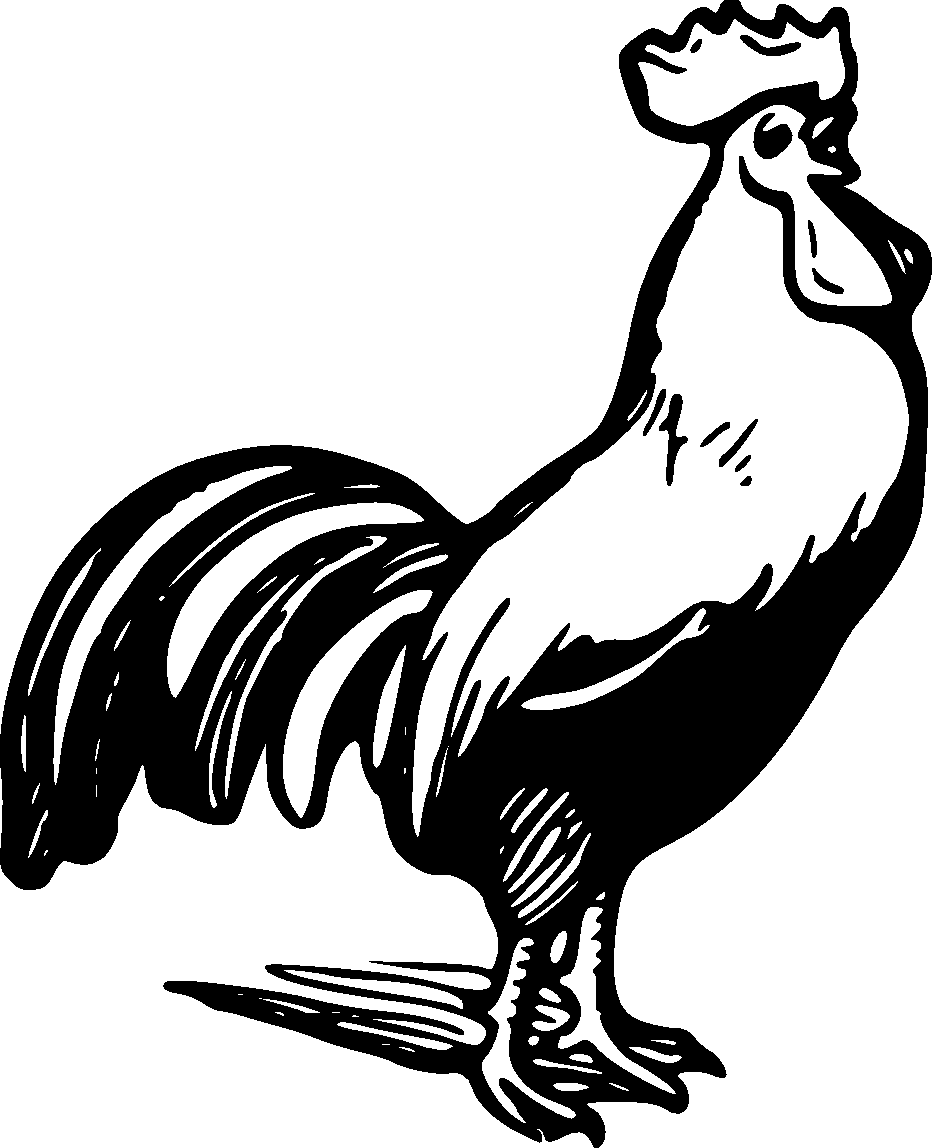
\includegraphics[height=0.9em]{coq.pdf}}
\newcommand{\CoqSymbol}{\raisebox{-.2ex}{\BareCoqSymbol\,}}
\newcommand{\Coqed}{{\hfill\CoqSymbol}}

% defining theorem environments for their specialized versions
\makeatletter
\newenvironment{base@thm}[4][\unskip]%
{\ifx\paslistend\undefined\else\global\let\paslistend\undefined\fi%
  $\;$\linebreak\noindent\mbox{$\triangleright\;\textsc{\textbf{\large #2} #3 (#4) #1.}$}}
{\hfill$\;$\linebreak}
\makeatother

% example environments take a label and a name
\crefname{example}{example}{examples}
\makeatletter
\newenvironment{example}[2][\unskip]%
{\refstepcounter{example}\begin{base@thm}[#1]{Example}{\theexample}{#2}}
{\end{base@thm}\noindent}
% referencing an example
\newcommand{\examplelabel}[2][PLACEHOLDER]{{#1}\label[example]{example:#2}\def\@currentlabel{#1}\label{t@example:#2}}
%\def\@currentlabel{#1}\label{t@example:#2}}
\newcommand{\exampleref}[1]{\Cref{example:#1}~(\ref{t@example:#1})}
\makeatother
% definition environments take a label and a name
\crefname{definition}{definition}{definitions}
\makeatletter
\newenvironment{definition}[2][\unskip]%
{\refstepcounter{definition}\begin{base@thm}[#1]{definition}{\thedefinition}{#2}}
{\end{base@thm}\noindent}
% referencing an definition
\newcommand{\definitionlabel}[2][PLACEHOLDER]{{#1}\label[definition]{definition:#2}\def\@currentlabel{#1}\label{t@definition:#2}}
%\def\@currentlabel{#1}\label{t@definition:#2}}
\newcommand{\definitionref}[1]{\Cref{definition:#1}~(\ref{t@definition:#1})}
\newcommand{\defref}[1]{\Cref{definition:#1}}
\makeatother
% lemma environments take a label and a name
\crefname{lemma}{lemma}{lemmas}
\makeatletter
\newenvironment{lemma}[2][\unskip]%
{\refstepcounter{lemma}\begin{base@thm}[#1]{lemma}{\thelemma}{#2}}
{\end{base@thm}\noindent}
% referencing an lemma
\newcommand{\lemmalabel}[2][PLACEHOLDER]{{#1}\label[lemma]{lemma:#2}\def\@currentlabel{#1}\label{t@lemma:#2}}
%\def\@currentlabel{#1}\label{t@lemma:#2}}
\newcommand{\lemmaref}[1]{\Cref{lemma:#1}~(\ref{t@lemma:#1})}
\newcommand{\lemref}[1]{\Cref{lemma:#1}}
\makeatother
% corollary environments take a label and a name
\crefname{corollary}{corollary}{corollarys}
\makeatletter
\newenvironment{corollary}[2][\unskip]%
{\refstepcounter{corollary}\begin{base@thm}[#1]{corollary}{\thecorollary}{#2}}
{\end{base@thm}\noindent}
% referencing an corollary
\newcommand{\corollarylabel}[2][PLACEHOLDER]{{#1}\label[corollary]{corollary:#2}\def\@currentlabel{#1}\label{t@corollary:#2}}
%\def\@currentlabel{#1}\label{t@corollary:#2}}
\newcommand{\corollaryref}[1]{\Cref{corollary:#1}~(\ref{t@corollary:#1})}
\makeatother
% axiom environments take a label and a name
\crefname{axiom}{axiom}{axioms}
\makeatletter
\newenvironment{axiom}[2][\unskip]%
{\refstepcounter{axiom}\begin{base@thm}[#1]{axiom}{\theaxiom}{#2}}
{\end{base@thm}\noindent}
% referencing an axiom
\newcommand{\axiomlabel}[2][PLACEHOLDER]{{#1}\label[axiom]{axiom:#2}\def\@currentlabel{#1}\label{t@axiom:#2}}
%\def\@currentlabel{#1}\label{t@axiom:#2}}
\newcommand{\axiomref}[1]{\Cref{axiom:#1}~(\ref{t@axiom:#1})}
\makeatother

% proofs
\crefname{asm}{assumption}{assumptions}
\crefname{goal}{goal}{goals}

%%% stack of passumptions 
\newtoks\passumptionsliststack
\passumptionsliststack={\empty}

\def\pushpassumptionsliststack#1#2{%
  \edef\tmp{{#1}\the#2}%
  #2=\expandafter{\tmp}%
}

\def\poppassumptionsliststack#1#2{%
  \expandafter\splitpassumptionsliststack\the#1\stop{#1}{#2}%
}

\def\splitpassumptionsliststack#1#2\stop#3#4{% 
  \def\tmp{#1}%
  \ifx\tmp\empty
  \else
    \def#4{#1}\global#3={#2}%
  \fi
} 
%%% stack of passumptions

\newlist{passumptionslist}{enumerate}{1}
\setlist[passumptionslist]{label=(\alph*)}

\newenvironment{assumptions}
    {\ifx\paslistend\undefined\else\global\let\paslistend\undefined\fi%
      \begin{passumptionslist}[start=1]
    }
    {
    \end{passumptionslist}
  }
\NoIndentAfterEnv{assumptions}
\newenvironment{goals}
    {\begin{enumerate}[label=(\roman*)]
    }
    {
    \end{enumerate}
  }
\NoIndentAfterEnv{goals}

\newcommand{\IH}[1][]{I{\kern-1.5pt}H#1}
\newenvironment{passumptions}[1][H]
  {%\thepassumptionslisti
  \ifx\paslistend\undefined%
    %{\color{red}\Large \thepassumptionslisti}
  \begin{passumptionslist}[resume*,label={$\left(#1_{\arabic*}\right)$}]%
  \else%
    %{\color{red}\Large \thepassumptionslisti === \paslistend}
  \begin{passumptionslist}[resume*,label={$\left(#1_{\arabic*}\right)$},start=\paslistend]%
  \global\let\paslistend\undefined%
  \fi%
  }
  {%
  \end{passumptionslist}%
  }
\NoIndentAfterEnv{passumptions}
% individual cases
\newcommand{\asm}[2]{\item\label[asm]{asm:#1} {$#2$}}
\newcommand{\goal}[2]{\item\label[goal]{goal:#1} {$#2$}}
\newcommand{\asmref}[1]{\Cref{asm:#1}}
\newcommand{\goalref}[1]{\Cref{goal:#1}}
% case environment
\makeatletter
\newenvironment{proofcase}[2][Case ]{%
    \global\edef\passumptionsliststackname{\thepassumptionslisti}%
    \pushpassumptionsliststack{\passumptionsliststackname}{\passumptionsliststack}%
    \par\noindent\ignorespaces%
    {\fbox{\textbf{#1}{$ #2 $}\textbf{:}}} %
    \begin{mdframed}[%
        topline=false,%
        rightline=false,%
        bottomline=false,%
        innertopmargin=0.2em,%
        innerbottommargin=0.4em,%
        innerrightmargin=0.7em,%
        rightmargin=0.7em,%
        innerleftmargin=0.7em,%
        leftmargin=0.7em,%
        linewidth=.15em,%
    ]\@ifpackageloaded{lineno}{\internallinenumbers}{}%
    \setlength{\parindent}{0pt} %
}{%
    \end{mdframed}\ignorespacesafterend%
    \poppassumptionsliststack{\passumptionsliststack}{\passumptionsliststackname}%
    \ifx\paslistend\undefined%
    \global\def\paslistend{\passumptionsliststackname+1}%
    \else%
    \global\def\paslistend{\passumptionsliststackname+1}%
    \fi%
    \setcounter{passumptionslisti}{\passumptionsliststackname}%
    %{\color{red}\Large\paslistend}
}
\makeatother
\NoIndentAfterEnv{proofcase}



% some cool operators
\newcommand{\isdef}[0]{\ensuremath{\mathrel{\overset{\makebox[0pt]{\mbox{\normalfont\tiny\sffamily def}}}{=}}}}

%% PL typesetting stuff 
% Lists
\newcommand{\mklist}[1]{\ensuremath\overline{#1}}
% Box explaining judgement
\newcommand{\textgraybox}[1]{\boxed{#1}}
\newdimen\zzfontsz
\newcommand{\fontsz}[2]{\zzfontsz=#1%
{\fontsize{\zzfontsz}{1.2\zzfontsz}\selectfont{#2}}}
\newcommand{\mathsz}[2]{\text{\fontsz{#1}{$#2$}}}
\newcommand{\instsymColon}{%
     \raisebox{-0.09ex}{\text{\normalfont{:}}}}
\newcommand{\judgboxfontsize}[1]{%
        \mathsz{11pt}{#1}%
}
\newcommand{\judgbox}[2]{%
      {\hrulefill\raggedright \textgraybox{\ensuremath{\judgboxfontsize{#1}}}\!\;%
        \fontsz{9pt}{\begin{tabular}[c]{l} #2 \end{tabular}\hrulefill} %
}}
\newcommand{\judgboxb}[2]{%
  \judgbox{#1}{#2}\hspace{1ex}\hrulefill%
}
\mdfdefinestyle{judgframe}{%
  topline=false, %
  innertopmargin=-2.84ex, %
  innerleftmargin=-.1ex, %
  innerrightmargin=0ex, %
  linewidth=.5pt %
}
\newcounter{judgements}
\crefname{judgements}{judgement}{judgements}
\newcommand{\judgementsref}[1]{\Cref{judgements:#1}}
\newenvironment{judgframe}[4][-2.84ex]
    {\begin{mdframed}[style=judgframe,innertopmargin=#1]\noindent%
      \judgbox{#3}{,,#4''}\def\thejudgements{\ensuremath{#3}}\refstepcounter{judgements}\label[judgements]{judgements:#2}\hrulefill\\[-0.9mm]%
      \begin{center}
    }
  {\end{center}%
   \end{mdframed}%
   \noindent%
  }
% Typerules
\newcounter{typerule}
\crefname{typerule}{rule}{rules}
% separator (may be different depending on used package, so its a macro)
\newcommand{\rulesep}{\qquad} %{\qquad\\\xspace}
\newcommand{\rulenewline}{\ensuremath \\\\}
% inductive predicates
\newcommand{\typeruleInt}[5]{%
	\def\thetyperule{#1}%
	\refstepcounter{typerule}%
	\label{tr:#4}%
	%
  %\ensuremath{\begin{array}{c}#5 \inference{#2}{#3}\end{array}}
  \ensuremath{\inferrule{ #2 }{ #3 }\quad #5}
}
\newcommand{\typerule}[4]{%
  \typeruleInt{#1}{#2}{#3}{#4}{\textsf{\scriptsize ({#1})}  }
}
\newcommand{\typerulenolabel}[2]{%
  \ensuremath{\inferrule{ #1 }{ #2 }}
}
\newcommand{\typederivX}[4][Right]{%
  %\ensuremath{\begin{array}{c} \inference{#2}{#3} #1\end{array}}
  \ensuremath{\inferrule*[#1=\textsc{\scriptsize(#2)}]{ #3 }{ #4 }}
}
\newcommand{\typederiv}[4][Right]{\typederivX[#1]{\trref{#2}}{#3}{#4}}
\newcommand{\asmderiv}[4][Right]{%
  %\ensuremath{\begin{array}{c} \inference{#2}{#3} #1\end{array}}
  \ensuremath{\inferrule*[#1=\textsc{\scriptsize(\asmref{#2})}]{ #3 }{ #4 }}
}
\newcommand{\lemderiv}[3]{%
  %\ensuremath{\begin{array}{c} \inference{#2}{#3} #1\end{array}}
  \ensuremath{\inferrule*[Right=\textsc{\scriptsize(\lemref{#1})}]{ #2 }{ #3 }}
}
%%%%%%%
% coinductive predicates
\newcommand{\cotyperuleInt}[5]{%
	\def\thetyperule{#1}%
	\refstepcounter{typerule}%
	\label{tr:#4}%
	%
  %\ensuremath{\begin{array}{c}#5 \inference{#2}{#3}\end{array}}
  \ensuremath{\mprset{fraction={===}}\inferrule{ #2 }{ #3 }~#5}
}
\newcommand{\cotyperule}[4]{%
  \cotyperuleInt{#1}{#2}{#3}{#4}{\textsf{\scriptsize ({#1})}  }
}
\newcommand{\cotyperulenolabel}[3]{%
	\def\thetyperule{#1}%
	\refstepcounter{typerule}%
  %\ensuremath{\begin{array}{c} \inference{#2}{#3}\end{array}}
  \ensuremath{\coinferrrule{ #2 }{ #3 }}
}
\newcommand{\cotyperulederiv}[3]{%
  %\ensuremath{\begin{array}{c} \inference{#2}{#3} #1\end{array}}
  \ensuremath{\mprset{fraction={===}}\inferrule{ #2 }{ #3 }~\textsc{(#1)}}
}
% referencing a rule
\newcommand{\trref}[1]{\Cref{tr:#1}}
\newcommand{\trrefshandler}[1]{,tr:#1}
\DeclareListParser*\forsemicolonlist{;}
\newcommand{\trrefs}[1]{\Cref{\forsemicolonlist\trrefshandler{#1}}}

% sandwiching
\newcommand{\lift}[1]{\ensuremath\lfloor\xspace{#1}\xspace\rfloor}
\newcommand{\hole}[1]{\ensuremath{\left[#1\right]}}
\newcommand{\denot}[1]{\ensuremath\left\llbracket#1\right\rrbracket\xspace}
\newcommand{\lrpars}[1]{\ensuremath\left(#1\right)\xspace}
\newcommand{\lrbrackets}[1]{\ensuremath\left[#1\right]\xspace}
\newcommand{\lrbraces}[1]{\ensuremath\left\{#1\right\}\xspace}
\newcommand{\lrbbraces}[1]{\ensuremath\left\llbracket{#1}\right\rrbracket\xspace}

%\newcommand{\tup}[2]{\ensuremath (#1 %
%  \readlist\myterms{#2}%
%  \foreachitem\x\in\myterms{;\x}%
%  )%
%}

%%%%%%%%%%%%%%%%%%%%%%%%%%%%%%%%
%% Properties Names
\newcommand{\tmssafe}{\text{tms}}
\newcommand{\smssafe}{\text{sms}}
\newcommand{\mssafe}{\text{ms}}
\newcommand{\ctsafe}{\text{ct}}
\newcommand{\scctsafe}{\text{sct}}
\newcommand{\msscctsafe}{\text{mssct}}
\newcommand{\sssafe}{\text{ss}}
\newcommand{\specmssafe}{\text{specms}}


%%
\newcommand{\emptyevent}{\ensuremath \varepsilon}
\newcommand{\ev}[1]{\ensuremath\ulcorner #1 \urcorner}
\newcommand{\tmsev}[1]{\ensuremath\ulcorner #1 \urcorner\;^{\kern-3pt{\tmssafe}}}
\newcommand{\smsev}[1]{\ensuremath\ulcorner #1 \urcorner\;^{\kern-3pt{\smssafe}}}
\newcommand{\msev}[1]{\ensuremath\ulcorner #1 \urcorner\;^{\kern-3pt{\mssafe}}}
\newcommand{\scctev}[1]{\ensuremath\ulcorner #1 \urcorner\;^{\kern-3pt{\scctsafe}}}
\newcommand{\specev}[1]{\ensuremath\ulcorner #1 \urcorner\;^{\kern-3pt{\sssafe}}}
\newcommand{\seqctev}[1]{\ensuremath\ulcorner #1 \urcorner\;^{\kern-3pt{\text{seq}}}_{\kern-3pt\ctsafe}}
\newcommand{\specctev}[1]{\ensuremath\ulcorner #1 \urcorner\;^{\kern-3pt{\text{spec}}}_{\kern-3pt\ctsafe}}
\newcommand{\seqarchev}[1]{\ensuremath\ulcorner #1 \urcorner\;^{\kern-3pt{\text{seq}}}_{\kern-3pt\text{arch}}}
\newcommand{\specarchev}[1]{\ensuremath\ulcorner #1 \urcorner\;^{\kern-3pt{\text{spec}}}_{\kern-3pt\text{arch}}}
\newcommand{\seqmemev}[1]{\ensuremath\ulcorner #1 \urcorner\;^{\kern-3pt{\text{seq}}}_{\kern-3pt\text{mem}}}
\newcommand{\specmemev}[1]{\ensuremath\ulcorner #1 \urcorner\;^{\kern-3pt{\text{spec}}}_{\kern-3pt\text{mem}}}

\newcommand{\lock}{\ensuremath\text{\scriptsize\faIcon{lock}}}
\newcommand{\unlock}{\ensuremath\text{\scriptsize\faIcon{lock-open}}}

\newcommand{\emptyTrace}{\ensuremath\hole{\cdot}}
\newcommand{\consTrace}[2]{\ensuremath{#1},{#2}}

\newcommand{\xlangrel}[2]{\ensuremath\sim^{#1}_{#2}}
\newcommand{\xlangreltr}[2]{\ensuremath\approx^{#1}_{#2}}

\newcommand{\seqctTOspecct}[2]{\xlangrel{seqct\kern2pt\lrpars{#1}}{specct\kern2pt\lrpars{#2}}}
\newcommand{\seqctTOspeccttr}[2]{\xlangreltr{seqct\kern2pt\lrpars{#1}}{specct\kern2pt\lrpars{#2}}}
\newcommand{\seqmemTOspecmem}[2]{\xlangrel{seqmem\kern2pt\lrpars{#1}}{specmem\kern2pt\lrpars{#2}}}
\newcommand{\seqmemTOspecmemtr}[2]{\xlangreltr{seqmem\kern2pt\lrpars{#1}}{specmem\kern2pt\lrpars{#2}}}
\newcommand{\seqarchTOspecarch}[2]{\xlangrel{seqarch\kern2pt\lrpars{#1}}{specarch\kern2pt\lrpars{#2}}}
\newcommand{\seqarchTOspecarchtr}[2]{\xlangreltr{seqarch\kern2pt\lrpars{#1}}{specarch\kern2pt\lrpars{#2}}}

\newcommand{\specmemTOspecct}{\xlangrel{specmem}{specct}}


\newcommand{\trgFenceEv}[1]{\ensuremath\trg{#1}}

%% Language-Specific events
\newcommand{\makeConcreteEvent}[3]{\ensuremath\ev{\textnormal{#1}\;\lrpars{#2}}\;^{\kern-3pt{#3}}}

\newcommand{\msEvent}[1][]{\ensuremath \varEvent[_{\mssafe}#1]}
\newcommand{\msTrace}[1][]{\ensuremath \varTrace[_{\mssafe}#1]}
\newcommand{\msAlloc}[1][\varLoc;n]{\ensuremath\makeConcreteEvent{Alloc}{#1}{\mssafe}}
\newcommand{\msDealloc}[1][\varLoc]{\ensuremath\makeConcreteEvent{Dealloc}{#1}{\mssafe}}
\newcommand{\msUse}[1][\varLoc;n]{\ensuremath\makeConcreteEvent{Use}{#1}{\mssafe}}

\newcommand{\smsEvent}[1][]{\ensuremath \varEvent[_{\smssafe}#1]}
\newcommand{\smsTrace}[1][]{\ensuremath \varTrace[_{\smssafe}#1]}
\newcommand{\smsAlloc}[1][\varLoc;n]{\ensuremath\makeConcreteEvent{Alloc}{#1}{\smssafe}}
\newcommand{\smsDealloc}[1][\varLoc]{\ensuremath\makeConcreteEvent{Dealloc}{#1}{\smssafe}}
\newcommand{\smsUse}[1][\varLoc;m]{\ensuremath\makeConcreteEvent{Use}{#1}{\smssafe}}

\newcommand{\tmsEvent}[1][]{\ensuremath \varEvent[_{\tmssafe}#1]}
\newcommand{\tmsTrace}[1][]{\ensuremath \varTrace[_{\tmssafe}#1]}
\newcommand{\tmsAlloc}[1][\varLoc]{\ensuremath\makeConcreteEvent{Alloc}{#1}{\tmssafe}}
\newcommand{\tmsDealloc}[1][\varLoc]{\ensuremath\makeConcreteEvent{Dealloc}{#1}{\tmssafe}}
\newcommand{\tmsUse}[1][\varLoc]{\ensuremath\makeConcreteEvent{Use}{#1}{\tmssafe}}

\newcommand{\scctEvent}[1][]{\ensuremath \varEvent[_{\scctsafe}#1]}
\newcommand{\scctTrace}[1][]{\ensuremath \varTrace[_{\scctsafe}#1]}
\newcommand{\scctAny}[1][\varSecuritytag]{\ensuremath\makeConcreteEvent{Any}{#1}{\scctsafe}}

\newcommand{\specEvent}[1][]{\ensuremath \varEvent[_{\mathghost}#1]}
\newcommand{\specTrace}[1][]{\ensuremath \varTrace[_{\mathghost}#1]}
\newcommand{\specAny}[1][\varSecuritytag]{\ensuremath\makeConcreteEvent{Any}{#1}{\mathghost}}

%% Language-Specific
\newcommand{\ctxtocomp}{\xspace ? \xspace}
\newcommand{\comptoctx}{\xspace ! \xspace}

\newcommand{\varLoc}[1][]{\ensuremath \ell_{#1}}
\newcommand{\varSecuritytag}[1][]{\ensuremath\sigma_{#1}}

\newcommand{\varWholeProg}[1][]{\ensuremath w_{#1}}
\newcommand{\varComponent}[1][]{\ensuremath p_{#1}}
\newcommand{\varContext}[1][]{\ensuremath C_{#1}}
\newcommand{\varRuntimeTerm}[1][]{\ensuremath r_{#1}}

\newcommand{\varEvent}[1][]{\ensuremath a_{#1}}
\newcommand{\varTrace}[1][]{\ensuremath \overline{a_{#1}}}
\newcommand{\varProperty}[1][]{\ensuremath \pi_{#1}}
\newcommand{\varHyperProperty}[1][]{\ensuremath \Pi_{#1}}
\newcommand{\varClass}[1][]{\ensuremath \mathbb{C}_{#1}}

\newcommand{\seqctEvent}[1][]{\ensuremath a^{\text{seq}}_{\text{ct}}\kern-3pt{#1}}
\newcommand{\specctEvent}[1][]{\ensuremath a^{\text{spec}}_{\text{ct}}\kern-3pt{#1}}
\newcommand{\seqmemEvent}[1][]{\ensuremath a^{\text{seq}}_{\text{mem}}\kern-3pt{#1}}
\newcommand{\specmemEvent}[1][]{\ensuremath a^{\text{spec}}_{\text{mem}}\kern-3pt{#1}}
\newcommand{\seqarchEvent}[1][]{\ensuremath a^{\text{seq}}_{\text{arch}}\kern-3pt{#1}}
\newcommand{\specarchEvent}[1][]{\ensuremath a^{\text{spec}}_{\text{arch}}\kern-3pt{#1}}

\newcommand{\seqctTrace}[1][]{\ensuremath \overline{a^{\text{seq}}_{\text{ct}}\kern-3pt{#1}}}
\newcommand{\specctTrace}[1][]{\ensuremath \overline{a^{\text{spec}}_{\text{ct}}\kern-3pt{#1}}}
\newcommand{\seqmemTrace}[1][]{\ensuremath \overline{a^{\text{seq}}_{\text{mem}}\kern-3pt{#1}}}
\newcommand{\specmemTrace}[1][]{\ensuremath \overline{a^{\text{spec}}_{\text{mem}}\kern-3pt{#1}}}
\newcommand{\seqarchTrace}[1][]{\ensuremath \overline{a^{\text{seq}}_{\text{arch}}\kern-3pt{#1}}}
\newcommand{\specarchTrace}[1][]{\ensuremath \overline{a^{\text{spec}}_{\text{arch}}\kern-3pt{#1}}}


\newcommand{\varMonitor}[1][]{\ensuremath T_{#1}}
\newcommand{\tmsMonitor}[1][]{\ensuremath\varMonitor[\tmssafe]#1}
\newcommand{\smsMonitor}[1][]{\ensuremath\varMonitor[\smssafe]#1}
\newcommand{\msMonitor}[1][]{\ensuremath\varMonitor[\mssafe]#1}
\newcommand{\scctMonitor}[1][]{\ensuremath\varMonitor[\scctsafe]#1}
\newcommand{\msscctMonitor}[1][]{\ensuremath\varMonitor[\msscctsafe]#1}
\newcommand{\specMonitor}[1][]{\ensuremath\varMonitor[\sssafe]#1}
\newcommand{\specmsMonitor}[1][]{\ensuremath\varMonitor[\specmssafe]#1}
\newcommand{\dualMonitor}[1][]{\ensuremath\varMonitor[A;B]#1}

\newcommand{\noncrashMonitor}[1]{\ensuremath{{\,^\circ}#1}}

% language specific versions of above
%% src
\newcommand{\srcWholeProg}[1][]{\ensuremath \src{\varWholeProg[#1]}}
\newcommand{\srcComponent}[1][]{\ensuremath \src{\varComponent[#1]}}
\newcommand{\srcContext}[1][]{\ensuremath \src{\varContext[#1]}}
\newcommand{\srcRuntimeTerm}[1][]{\ensuremath \src{\varRuntimeTerm[#1]}}

\newcommand{\srcEvent}[1][]{\ensuremath \src{\varEvent[#1]}}
\newcommand{\srcTrace}[1][]{\ensuremath \src{\varTrace[#1]}}
\newcommand{\srcProperty}[1][]{\ensuremath \src{\varProperty[#1]}}
\newcommand{\srcHyperProperty}[1][]{\ensuremath \src{\varHyperProperty[#1]}}
\newcommand{\srcClass}[1][]{\ensuremath \src{\varClass[#1]}}
%% trg
\newcommand{\trgWholeProg}[1][]{\ensuremath \trg{\varWholeProg[#1]}}
\newcommand{\trgComponent}[1][]{\ensuremath \trg{\varComponent[#1]}}
\newcommand{\trgContext}[1][]{\ensuremath \trg{\varContext[#1]}}
\newcommand{\trgRuntimeTerm}[1][]{\ensuremath \trg{\varRuntimeTerm[#1]}}

\newcommand{\trgEvent}[1][]{\ensuremath \trg{\varEvent[#1]}}
\newcommand{\trgTrace}[1][]{\ensuremath \trg{\varTrace[#1]}}
\newcommand{\trgProperty}[1][]{\ensuremath \trg{\varProperty[#1]}}
\newcommand{\trgHyperProperty}[1][]{\ensuremath \trg{\varHyperProperty[#1]}}
\newcommand{\trgClass}[1][]{\ensuremath \trg{\varClass[#1]}}
%% irl
\newcommand{\irlWholeProg}[1][]{\ensuremath \irl{\varWholeProg[#1]}}
\newcommand{\irlComponent}[1][]{\ensuremath \irl{\varComponent[#1]}}
\newcommand{\irlContext}[1][]{\ensuremath \irl{\varContext[#1]}}
\newcommand{\irlRuntimeTerm}[1][]{\ensuremath \irl{\varRuntimeTerm[#1]}}

\newcommand{\irlEvent}[1][]{\ensuremath \irl{\varEvent[#1]}}
\newcommand{\irlTrace}[1][]{\ensuremath \irl{\varTrace[#1]}}
\newcommand{\irlProperty}[1][]{\ensuremath \irl{\varProperty[#1]}}
\newcommand{\irlHyperProperty}[1][]{\ensuremath \irl{\varHyperProperty[#1]}}
\newcommand{\irlClass}[1][]{\ensuremath \irl{\varClass[#1]}}

% bops
\newcommand{\bopLink}[2]{\ensuremath {#1}\bowtie{#2}}
\newcommand{\fncompo}[2]{\ensuremath {#1}\circ{#2}}

% different kinds of satifsaction
\newcommand{\sat}[2]{\ensuremath \vdash {#1} : {#2}}
\newcommand{\rsat}[2]{\ensuremath \vdash_R {#1} : {#2}}

\newcommand{\rtp}[2]{\ensuremath\;\vdash{#1}:{#2}}
\newcommand{\rtpUniversal}[3]{\ensuremath\;\vdash^{\forall}_{{#3}}{#1}:{#2}}
\newcommand{\rtpExistential}[3]{\ensuremath\;\vdash^{\exists}_{{#3}}{#1}:{#2}}


\newcommand{\progstepto}[3]{\ensuremath{#1}\xRightarrow{#3}{#2}}


\newcommand{\cc}[3][\gamma]{\ensuremath {#1}^{#2}_{#3}}
\newcommand{\ccST}[1][\gamma]{\ensuremath \cc[#1]{\src{S}}{\trg{T}}}
\newcommand{\ccSI}[1][\gamma]{\ensuremath \cc[#1]{\src{S}}{\irl{I}}}
\newcommand{\ccIT}[1][\gamma]{\ensuremath \cc[#1]{\irl{I}}{\trg{T}}}
\newcommand{\ccII}[1][\gamma]{\ensuremath \cc[#1]{\irl{I}}{\irl{I}}}


\newcommand{\mapUniversal}[2]{\ensuremath \overset{#1}{\varsigma}\left({#2}\right)}
\newcommand{\mapExistential}[2]{\ensuremath \overset{#1}{\tau}\left({#2}\right)}
\newcommand{\xrelTraces}[2]{\ensuremath {#1}\sim{#2}}


\newcommand{\mapUniversalWF}[2]{\ensuremath \vdash {#1} : \mathit{WF}^{\forall}_{#2}}
\newcommand{\mapExistentialWF}[2]{\ensuremath \vdash {#1}\ ; \mathit{WF}^{\exists}_{#2}}


% Reductions
\usetikzlibrary{calc,decorations.pathmorphing,shapes}

\newcounter{sarrow}
\newcommand\xrsquigarrow[1]{%
\stepcounter{sarrow}%
\mathrel{\begin{tikzpicture}[baseline= {( $ (current bounding box.south) + (0,-0.5ex) $ )}]
\node[inner sep=.5ex] (\thesarrow) {$\scriptstyle #1$};
\path[draw,<-,decorate,
  decoration={zigzag,amplitude=0.7pt,segment length=1.2mm,pre=lineto,pre length=4pt}] 
    (\thesarrow.south east) -- (\thesarrow.south west);
\end{tikzpicture}}%
}
\newcommand{\monitorcheck}[4][{\kern-3.5pt}^*]{%
  \vdash\xspace{#2}\xspace \xrsquigarrow{#4}{#1}\xspace{#3}\xspace%
}


